\documentclass{rvcepaper}
\begin{document}

% ---------- HS261TA Principles of Management & Economics
\begin{iempaper}
\paperinfo{shownote=0,date={22/05/2026},exam={CIE -- 2},maxmarks={10 + 50},sem={VI},prog={UG},duration={30 + 90 Min},
 title={Principles of Management\& Economics},code={HS261TA}}
\iemhead
{\small Note:}\par\vspace{-1pt}
\hspace*{0.5cm}{\footnotesize 1. \hspace{0.1cm}Answer all the Questions.}\par\vspace{3pt}
\begin{cietable}{M}{BT}{CO}
\qpart{Part -- A}
\q{1.}{In the BCG matrix, what does a ``Star'' represent? Why is it important for a company?}{02}{2}{CO2}
\q{2.}{Differentiate Strategic and Operational plans on the basis of time horizons.}{02}{2}{CO2}
\q{3.}{Give two examples of corporate level strategy}{02}{2}{CO2}
\q{4.}{When price of a product falls from \rupee 20 to \rupee 16, quantity demanded rises from 100 units to 140 units. Find Price Elasticity of Demand.}{02}{3}{CO3}
\q{5.}{If the total cost of the basket in the base period (say January 2008) is \$600, and in the current period (say February 2008) it is \$616, calculate the CPI.}{02}{3}{CO3}
\qpart{Part -- B}
\q{1.}{The rapid growth of electric vehicles (EVs) in India has increased the demand for skilled EV technicians and battery maintenance experts. However, the limited availability of trained workers resulted in higher wages, labor shortages, and delays in service operations. To overcome this challenge, companies and the government introduced training and skill development programs to increase the supply of skilled labor.\newline
Analyze the impact of demand and supply forces on:\newline
a) Wages of EV technicians\newline
b) Employment opportunities\newline
c) Labor shortages in the EV sector\newline
d) Skill development initiatives}{10}{4}{CO4}
\q{2.}{The caf\'e industry in Bengaluru has become highly competitive due to the increasing number of caf\'es offering similar products such as coffee and snacks. To attract customers, caf\'es differentiate themselves through ambience, branding, pricing, customer service, and promotional activities. ``Urban Brew Caf\'e,'' which initially enjoyed high profits, has started losing customers after the entry of new competitors offering attractive pricing and unique customer experiences. As a result, the caf\'e faces challenges in maintaining profitability and customer loyalty in a monopolistically competitive market.\newline
Based on the above case, discuss the role of monopolistic competition in business performance with reference to:\newline
a) Product differentiation and its impact on profit\newline
b) Advertising strategies used to attract customers\newline
c) Pricing strategies adopted by caf\'es\newline
d) Techniques for business survival in a competitive market}{10}{4}{CO4}
\q{3.}{a\quad Illustrate the Oligopoly's version of the prisoner's dilemma with an example.\newline\newline
b\quad What is the expected economic impact of Budget 2026?}{05\newline\newline 05}{2\newline\newline 2}{CO2\newline\newline CO2}
\q{4.}{India's electric vehicle (EV) industry is experiencing rapid growth due to government initiatives like FAME-II, rising fuel prices, and increasing environmental awareness. However, companies operating in this sector face challenges such as inadequate charging infrastructure, dependency on imported lithium-ion batteries, intense competition from domestic and global players, and rapidly changing technology. In this context, analyze how an Indian EV manufacturing company can use strategic planning to achieve sustainable growth, improve market share, and ensure long-term competitiveness in the evolving Indian automotive industry.}{10}{4}{CO4}
\q{5.}{Zeta Pharma, a Hyderabad-based pharmaceutical company supplying essential medicines across India, faced a sudden crisis in 2026 when geopolitical trade restrictions disrupted the import of a key raw material used in a life-saving drug. With only limited stock available, the company risked stopping production within weeks, affecting hospitals and patients nationwide. Since no standard procedure existed for such a disruption, top management had to take non-programmed managerial decisions under uncertainty. They evaluated options such as expensive emergency imports, prioritizing critical drug production, and collaborating with competitors or government agencies. The situation required quick judgment, risk analysis, and strategic thinking to ensure uninterrupted medicine supply.\newline
Give the analysis of the Risk analysis and strategic thinking to be adopted in the case.}{10}{4}{CO4}
\end{cietable}
\end{iempaper}

% ---------- IM362IA Supply Chain Management
\begin{iempaper}
\paperinfo{shownote=0,date={26.05.2026},exam={CIE -- II},maxmarks={10 + 50},sem={VI},prog={UG},duration={30 + 90 Min},
 title={Supply Chain Management},code={IM362IA}}
\iemhead
{\small Note:}\par\vspace{-1pt}
\hspace*{0.5cm}{\footnotesize 1. \hspace{0.1cm}Answer all the Questions.}\par
\hspace*{0.5cm}{\footnotesize 2. \hspace{0.1cm}Use of Normal Distribution Tables permitted.}\par\vspace{3pt}
\begin{cietable}{M}{BT}{CO}
\qpart{Part -- A}
\q{1.}{What is the inference drawn from this figure?
\par\vspace{2pt}\noindent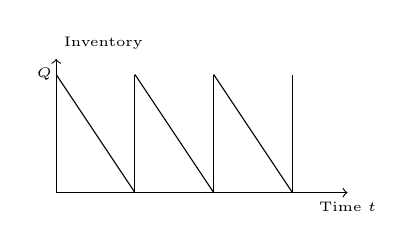
\begin{tikzpicture}[x=0.5cm,y=0.5cm,font=\tiny]
\draw[->] (0,0) -- (0,3.4) node[above,xshift=0.6cm] {Inventory}; \draw[->] (0,0) -- (7.4,0) node[below] {Time $t$};
\draw (0,3) -- (2,0); \draw (2,3) -- (4,0); \draw (4,3) -- (6,0); \draw (2,0) -- (2,3); \draw (4,0) -- (4,3); \draw (6,0) -- (6,3);
\node at (-0.3,3) {$Q$};
\end{tikzpicture}\par}{2}{2}{CO3}
\q{2.}{The primary role of cycle inventory is to allow different stages in the supply chain to purchase product in lot sizes that minimize the sum of the \blank[3.2cm], \blank[1.9cm], and \blank[1.9cm] cost.}{2}{1}{CO3}
\q{3.}{A key to reducing lot size without \blank[2.4cm] costs is to \blank[2.4cm] the fixed cost associated with each lot.}{2}{1}{CO2}
\q{4.}{What is intermodal transportation?}{2}{1}{CO2}
\q{5.}{Identify the transportation design option that is illustrated in the sketch. List one application of this design.
\par\vspace{4pt}\noindent\begin{tikzpicture}[x=1cm,y=1cm,font=\tiny]
\foreach \i in {0,...,5} {\draw (\i*0.85,2.4) circle (0.32);}
\node[right] at (4.5,2.7) {Suppliers};
\foreach \i in {0,...,5} {\draw[rounded corners=2pt] (\i*0.85-0.2,0.1) rectangle (\i*0.85+0.2,0.7);}
\foreach \i in {1,...,5} {\draw[-{Stealth}] (\i*0.85-0.2,0.4) -- (\i*0.85-0.65,0.4);}
\foreach \i in {0,...,4} {\draw[dashed] (4.25,2.1) -- (\i*0.85,0.7);}
\draw[-{Stealth}] (4.25,2.1) -- (4.25,0.7);
\node at (5.6,0.4) {Buyer Locations};
\end{tikzpicture}\par}{2}{2}{CO2}
\qpart{Part - B}
\q{1}{With a help of suitable case example elucidate tailored transportation decision made based on size of customer.}{10}{2}{CO2}
\q{2}{Discuss trade-offs in transportation design with examples.}{10}{2}{CO2}
\q{3}{Demand for the Deskpro computer at Best Buy is 1,000 units per month. Best Buy incurs a fixed order placement, transportation, and receiving cost of \$4,000 each time an order is placed. Each computer costs Best Buy \$500 and the retailer has a holding cost of 20 percent. Evaluate the number of computers that the store manager should order in each replenishment lot, number of orders per year, annual inventory cost, and average flow time.}{10}{3}{CO3}
\q{4}{Weekly demand for HP printers at a Sam's Club store is normally distributed, with a mean of 250 and a standard deviation of 150. The store manager continuously monitors inventory and currently orders 1,000 printers each time the inventory drops to 600 printers. HP currently takes two weeks to fill an order. How much safety inventory does the store carry as a result of this policy? What fill rate does the store achieve? Assume that the supply lead time from HP is normally distributed, with a mean of 2 weeks and a standard deviation of 1.5 weeks. How much safety inventory should Sam's Club carry if it wants to provide a CSL of 95 percent?}{10}{3}{CO3}
\q{5}{Assume that weekly demand for phones at B\&M Office Supplies is normally distributed, with a mean of 2,500 and a standard deviation of 500. The manufacturer takes two weeks to fill an order placed by the B\&M manager. The store manager currently orders 10,000 phones when the inventory on hand drops to 6,000. Evaluate the safety inventory and the average inventory carried by B\&M. Also evaluate the average time a phone spends at B\&M.\newline
Weekly demand for Legos at a Wal-Mart store is normally distributed, with a mean of 2,500 boxes and a standard deviation of 500. The replenishment lead time is two weeks. Assuming a continuous review replenishment policy, evaluate the safety inventory that the store should carry to achieve a CSL of 90 percent.}{05\newline\newline\newline\newline\newline\newline\newline 05}{4}{CO3}
\end{cietable}
\end{iempaper}

% ---------- IM363IA Ergonomics
\begin{iempaperB}
\paperinfo{hdr=2,usn=0,ayear={2025-2026(Even Sem)},date={25\textsuperscript{th} MAY 2026},code={IM363IA},sem={VI Semester},exam={Test-2},maxmarks={50},duration={90 Min},
 title={ERGONOMICS},shownote=0,yearword={year}}
\iemheadB
\ptitle{PART A}
\begin{xtable}{Questions}
\q{1}{How does repetitive motion contribute to musculoskeletal disorders?}{02}{L2}{2}
\q{2}{Define moment arm in the context of biomechanics.}{02}{L1}{3}
\q{3}{List any two types of controls used in human-machine systems.}{02}{L2}{4}
\q{4}{Differentiate between discrete controls and continuous controls.}{02}{L2}{2}
\q{5}{What are labels and icons in display design?}{02}{L2}{2}
\end{xtable}
\ptitle{PART B}
\begin{xtable}{Questions}
\q{1}{Design an ergonomic human-machine interface for a workplace of your choice by integrating suitable displays, controls, icons, labels, and navigation aids. Justify your design decisions based on ergonomic principles.}{10}{L4}{1}
\q{2}{Analyse the ergonomic risks associated with poorly designed displays and controls in workplaces. Discuss how improper interface design can contribute to work-related musculoskeletal disorders (WMSDs).}{10}{L3}{3}
\q{3}{Explain the different types of displays used in ergonomics and discuss the major tasks performed through displays in human-machine systems. Illustrate the role of monitoring displays and integrative displays with suitable examples.}{10}{L3}{1}
\q{4}{Describe the major causes of low back problems in workplaces. Explain the ergonomic risk factors that contribute to lower back injuries among workers.}{10}{L2}{3}
\q{5}{A worker in a warehouse repeatedly lifts heavy boxes from the floor to shoulder height. Using ergonomic principles and the NIOSH lifting guide, analyse the risks involved and suggest suitable ergonomic improvements.}{10}{L4}{2}
\end{xtable}
\btfoot{|l|l|l|*{11}{C{0.8cm}|}}{\hline
\multirow{2}{*}{\shortstack{Marks\\Distribution}} & \multicolumn{2}{c|}{Particulars} & CO1 & CO2 & CO3 & CO4 & CO5 & L1 & L2 & L3 & L4 & L5 & L6\\\cline{2-14}
 & Max & Quiz & & 06 & 02 & 02 & & 02 & 08 & & & & \\\cline{3-14}
 & Marks & Test & 20 & 10 & 20 & & & & 10 & 30 & 10 & & \\\hline}
\end{iempaperB}

% ---------- IM364TA Human Resource Management & Analytics
\begin{iempaperB}
\paperinfo{hdr=2,usn=0,ayear={2025 - 26 (EVEN Sem)},dept={INDUSTRIAL ENGINEERING \& MANAGEMENT},date={26\textsuperscript{th} May 2026},code={IM364TA},sem={VI Semester},exam={CIE -- II},maxmarks={10 + 50},duration={120 Min},
 title={Human Resource Management \& Analytics - IM364TA},shownote=0}
\iemheadB
\ptitle{Part -- A}
\begin{xtable}{Questions}
\q{1.}{Distinguish between \textit{predictive validity} and \textit{concurrent validity}.}{01}{L1}{CO2}
\q{2.}{Define \textit{negligent hiring} in the context of HR selection.}{01}{L1}{CO2}
\q{3.}{What is meant by \textit{validity} in employee testing?}{01}{L1}{CO2}
\q{4.}{What is an \textit{in-basket exercise}?}{01}{L2}{CO3}
\q{5.}{Differentiate between orientation and onboarding.}{01}{L1}{CO3}
\q{6.}{What is on-the-job training?}{01}{L1}{CO3}
\q{7.}{Define appraisal interview.}{01}{L1}{CO3}
\q{8.}{Define graphic rating scale in performance appraisal}{01}{L2}{CO3}
\q{9.}{What is succession planning in talent management}{01}{L2}{CO3}
\q{10.}{A company identifies a gap between employee skills and job requirements. What is the first step in the training process?}{01}{L2}{CO3}
\end{xtable}
\ptitle{Part -- B}
\begin{xtable}{Questions}
\q{1.}{List and describe eight types of employment tests used in employee selection. For each type, state: (i) what it measures, and (ii) the category of jobs or employees for which it is most suitable.}{10}{L2}{CO2}
\q{2.}{A multinational company is selecting candidates for a middle management role. Design a Management Assessment Centre for this role. Specify at least three simulations, the managerial competency each exercise measures, and how assessors should evaluate candidate performance in each exercise.}{10}{L3}{CO2}
\q{3.}{A bank introduced digital banking services, but employees lacked the technical skills to operate the new system effectively. Develop a suitable training program to help employees adapt to the technological changes.}{10}{L3}{CO3}
\q{4.}{A service organization plans to evaluate employee performance using feedback from supervisors, peers, subordinates, and customers. Recommend a suitable appraisal technique and explain how it can be implemented effectively.}{10}{L3}{CO3}
\q{5.}{Employees in a company often become defensive during appraisal interviews and fail to accept feedback positively. Develop guidelines for managers to conduct effective appraisal interviews that encourage employee improvement.}{10}{L3}{CO3}
\end{xtable}
\btfoot{|l|l|l|*{10}{C{0.85cm}|}}{\hline
\multirow{2}{*}{Marks Distribution} & \multicolumn{2}{c|}{Particulars} & CO1 & CO2 & CO3 & CO4 & L1 & L2 & L3 & L4 & L5 & L6\\\cline{2-13}
 & Quiz & Max Marks & -- & 04 & 06 & -- & 06 & 04 & -- & -- & -- & --\\\cline{2-13}
 & Test & Max Marks & -- & 20 & 30 & -- & -- & 10 & 40 & -- & -- & --\\\hline}
\stars{***********}
\end{iempaperB}

% ---------- IM365TDA Facilities Planning And Design
\begin{iempaper}
\paperinfo{shownote=0,date={25\textsuperscript{th} May 2026},exam={CIE -- II},maxmarks={10 + 50},sem={VI},prog={UG},duration={30 + 90 Min},
 title={Facilities Planning And Design (Professional Core Elective)},code={IM365TDA}}
\iemhead
{\small Note:}\par\vspace{-1pt}
\hspace*{0.5cm}{\footnotesize 1. \hspace{0.1cm}Answer all the Questions.}\par\vspace{3pt}
\begin{cietable}{M}{BT}{CO}
\qpart{Part -- A}
\q{1.}{State the main objectives of material handling?}{(02)}{1}{1}
\q{2.}{What is meant by unit load design?}{(02)}{2}{2}
\q{3.}{Enumerate the importance of flexibility in material handling systems.}{(02)}{3}{3}
\q{4.}{What is the role of conveyors in material handling?}{(02)}{2}{4}
\q{5.}{State two objectives of computer aided layout techniques.}{(02)}{2}{3}
\qpart{Part -- B}
\q{1.}{Discuss the scope of material handling in modern industries.}{(10)}{2}{2}
\q{2.}{Explain movement, time, quantity and space of a material handling system}{(10)}{3}{2}
\q{3.}{Explain the following cost components used in estimating material handling cost:
\begin{romi}\item Equipment cost\item Storage \& Inventory Costs\item Damage/Wastage Costs\end{romi}}{(10)}{3}{3}
\q{4.}{Explain the safety considerations to be followed in material handling operations.}{(10)}{3}{4}
\q{5.}{Consider the following data with unit cost matrix. Use CRAFT pair-wise interchange technique to obtain the desirable layout.\newline
Total number of departments: 4\newline
Total number of interchangeable departments: 4\newline
Initial Layout:
\par\vspace{2pt}\centerline{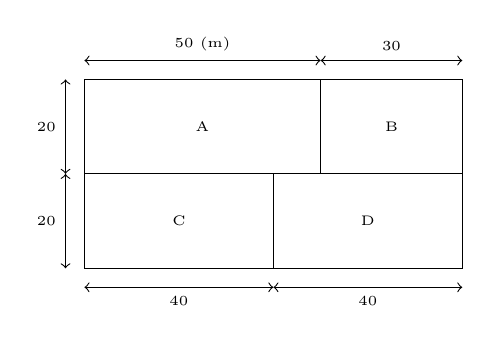
\begin{tikzpicture}[x=0.06cm,y=0.06cm,font=\tiny]
\draw (0,0) rectangle (80,40);\draw (0,20)--(80,20);\draw (50,20)--(50,40);\draw (40,0)--(40,20);
\node at (25,30) {A};\node at (65,30) {B};\node at (20,10) {C};\node at (60,10) {D};
\draw[<->] (0,44)--(50,44);\node[above] at (25,44) {50 (m)};\draw[<->] (50,44)--(80,44);\node[above] at (65,44) {30};
\draw[<->] (-4,20)--(-4,40);\node[left] at (-4,30) {20};\draw[<->] (-4,0)--(-4,20);\node[left] at (-4,10) {20};
\draw[<->] (0,-4)--(40,-4);\node[below] at (20,-4) {40};\draw[<->] (40,-4)--(80,-4);\node[below] at (60,-4) {40};
\end{tikzpicture}}\par\vspace{2pt}
Area of Departments (Scale 1000 sq units = 1 sq unit):
\qtab{|l|c|c|c|c|}{\hline Department & A & B & C & D\\\hline Area (sq. units) & 10 & 6 & 8 & 8\\\hline}
Flow Matrix:
\qtab{|c|c|c|c|c|}{\hline From$\backslash$To & A & B & C & D\\\hline A & -- & 2 & 4 & 4\\\hline B & 1 & -- & 1 & 3\\\hline C & 2 & 1 & -- & 2\\\hline D & 4 & 1 & 0 & --\\\hline}}{(10)}{2}{4}
\end{cietable}
\stars{********}
\end{iempaper}

% ---------- IM365TDB Service Operations Management
\begin{iempaper}
\paperinfo{shownote=0,date={25-05-2026},exam={CIE -- II},maxmarks={10 + 50},sem={VI},prog={UG},duration={30 + 90 Min},
 title={Service Operations Management},code={IM365TDB}}
\iemhead
{\small Note:}\par\vspace{-1pt}
\hspace*{0.5cm}{\footnotesize 1. \hspace{0.1cm}Answer all the Questions.}\par\vspace{3pt}
\begin{cietable}{M}{BT}{CO}
\qpart{Part -- A}
\q{1.}{Imagine you are going to watch an IPL cricket match at Namma Bengaluru's very own Chinnaswamy Cricket stadium, list 4 aspects that you associate regarding service experience.}{2}{1}{1}
\q{2.}{Assume you get in to an ``IT enabled service'' (ITES) industry in the next five years. Comment on how you intend to use Service as a competitive advantage.}{2}{4}{3}
\q{3.}{Assume you are being interviewed for your short but successful career in the field of ``Service operations management''. One of the questions from a young enthusiast is ``How to develop a culture of service quality in an organization?'' Comment any two aspects.}{2}{4}{2}
\q{4.}{Some of you have already started preparing for campus placements. In a year from now, many of your juniors would want your suggestions \textbf{(If placed)} and help in many matters of campus placements. To cater to this need and based on some of the requirement analysis that you have done, you wish to start a service and name it as ``\textbf{Placement war room}'' for engineering graduate students. Now answer the following questions.
\begin{num}\item Will it be online or offline and why?\item What are the unmet needs of graduate students that your service will fulfil?\end{num}}{2}{4}{4}
\q{5.}{If your ``\textbf{Placement war room}'' idea clicks and is appreciated by your initial target audience. Identify any 2-success metrics of your service? Also, comment on the possible perception expectation gap for your service.}{2}{4}{3}
\qpart{Part -- B}
\q{1}{Discuss the role of technology in developing the customer Experience. Cite two examples of services where technology has been used effectively to enhance customer experience.}{10}{3}{4}
\q{2}{The nature of supply chains can be very messy and complex. Describe the key issues service operations managers should focus on with a key focus on managing through intermediaries.}{10}{3}{4}
\q{3}{Write short notes on
\begin{abc}\item Service level agreements (SLA)\item Difference between SLA and Operational Level Agreements (OLA)\end{abc}}{5*2=10}{2}{3}
\q{4}{Envisage/visualize an experience map for a customer visiting a typical dental clinic.}{10}{4}{2}
\q{5}{One of the key decisions for procurement function is choosing/selecting a supply partner and particularly for those who handle critical elements of supply chain. Discuss the criteria for supplier selection excluding Cost and Quality.}{10}{3}{4}
\end{cietable}
\end{iempaper}

% ---------- IM365TDD Design of Experiments
\begin{iempaper}
\paperinfo{shownote=0,date={25/05/2026},exam={CIE -- II},maxmarks={10 + 50},sem={VI},prog={UG},duration={30 + 90 Min},
 title={Design of Experiments},code={IM365TDD}}
\iemhead
{\small Instructions to Students:}\par\vspace{-1pt}
\hspace*{0.5cm}{\footnotesize 1. \hspace{0.1cm}Answer all questions}\par
\hspace*{0.5cm}{\footnotesize 2. \hspace{0.1cm}Use of statistical tables permitted}\par\vspace{3pt}
\begin{cietable}{M}{BT}{CO}
\qpart{Part -- A}
\q{1.}{Define ``Sparsity of Effects Principle.''}{2}{1}{CO1}
\q{2.}{If you have a $2^5$ design, how many total treatment combinations are required for a single replicate?}{1}{1}{CO1}
\q{3.}{Compare the $2^2$ design and $3^2$ designs in terms of modeling.}{2}{1}{CO2}
\q{4.}{What is ``Confounding'' in factorial experiments?}{2}{2}{CO2}
\q{5.}{Define ``Aliasing'' in fractional factorial designs.}{1}{2}{CO2}
\q{6.}{Evaluate the risk of using a Resolution III design for a process where two-factor interactions are known to be significant.}{2}{2}{CO2}
\qpart{Part -- B}
\q{1}{An engineer is interested in the effects of cutting speed ($A$), tool geometry ($B$), and cutting angle ($C$) on the life (in hours) of a machine tool. Two levels of each factor are chosen, and three replicates of a $2^3$ factorial design are run. The results are as follows:
\qtabc{|c|c|c|c|c|c|c|}{\hline \multirow{2}{*}{$A$} & \multirow{2}{*}{$B$} & \multirow{2}{*}{$C$} & \multirow{2}{*}{\shortstack{Treatment\\Combination}} & \multicolumn{3}{c|}{Replicates}\\\cline{5-7} & & & & I & II & III\\\hline $-$ & $-$ & $-$ & (1) & 22 & 31 & 25\\\hline $+$ & $-$ & $-$ & a & 32 & 43 & 29\\\hline $-$ & $+$ & $-$ & b & 35 & 34 & 50\\\hline $+$ & $+$ & $-$ & ab & 55 & 47 & 46\\\hline $-$ & $-$ & $+$ & c & 44 & 45 & 38\\\hline $+$ & $-$ & $+$ & ac & 40 & 37 & 36\\\hline $-$ & $+$ & $+$ & bc & 60 & 50 & 54\\\hline $+$ & $+$ & $+$ & abc & 39 & 41 & 47\\\hline}
\begin{romi}\item Estimate the factor effects. Which effects appear to be large?\item Use the analysis of variance to confirm your conclusions for part (i).\end{romi}}{20}{2}{CO4}
\q{2}{The effects of developer strength ($A$) and development time ($B$) on the density of photographic plate film are being studied. Three strengths and three times are used, and four replicates of a $3^2$ factorial experiment are run. The data from this experiment follow. Analyze the data using the standard methods for factorial experiments.
\qtabc{|c|c|c|c|c|c|c|c|c|c|c|c|c|c|}{\hline \multicolumn{2}{|c|}{} & \multicolumn{12}{c|}{Development Time (minutes)}\\\cline{3-14} \multicolumn{2}{|c|}{} & \multicolumn{4}{c|}{10} & \multicolumn{4}{c|}{14} & \multicolumn{4}{c|}{18}\\\hline \multirow{3}{*}{\shortstack{Developer\\Strength}} & 1 & 0 & 2 & 1 & 3 & 2 & 5 & 4 & 4 & 2 & 3 & 2 & 5\\\cline{2-14} & 2 & 4 & 6 & 6 & 8 & 9 & 10 & 5 & 4 & 2 & 4 & 6 & 7\\\cline{2-14} & 3 & 7 & 7 & 5 & 7 & 7 & 8 & 5 & 7 & 10 & 8 & 9 & 12\\\hline}}{20}{3}{CO4}
\q{3}{List and explain the three key ideas / principles that are to be implemented for the successful use of fractional factorial designs.}{10}{2}{CO2}
\end{cietable}
\end{iempaper}

% ---------- IM266TEQ Elements of Financial Management
\begin{iempaperB}
\paperinfo{hdr=2,ayear={2025-2026 (EVEN Sem)},date={22 May 2026},code={IM266TEQ},sem={VI Semester},exam={CIE -- II},maxmarks={10 + 50},duration={120 Mins},
 title={ELEMENTS OF FINANCIAL MANAGEMENT (Institutional Elective)},shownote=0}
\iemheadB
{\small Note:}\par\vspace{-1pt}
\hspace*{0.5cm}{\footnotesize 1. \hspace{0.1cm}Answer all the Questions.}\par
\hspace*{0.5cm}{\footnotesize 2. \hspace{0.1cm}Use of Interest factor tables permitted.}\par\vspace{3pt}
\ptitle{PART -- A}
\begin{xtable}{Questions}
\q{1}{Distinguish between the terms, Risk and Return in Financial Management.}{2}{2}{2}
\q{2}{What is meant by ``Yield to Maturity'' (YTM) of a bond.}{2}{1}{2}
\q{3}{Mention the three key inputs required to perform the valuation of an Asset.}{2}{2}{2}
\q{4}{What is meant by Required Rate of Return in the context of valuation of securities.}{2}{2}{2}
\q{5}{Distinguish between the terms Market Risk and Unique Risk.}{2}{2}{2}
\end{xtable}
\ptitle{PART -- B}
\begin{xtable}{Questions}
\q{1.a}{Explain why a bond sells at a premium or discount.}{5}{4}{2}
\q{b}{A 5-year bond, coupon rate 8\%, par value \rupee 1,000, required return 10\%. Find bond price.}{5}{3}{2}
\q{2.a}{A bond has a par value \rupee 1,000, coupon rate 12\%, maturity 5 years, current price \rupee 950. Compute the Yield to Maturity (YTM).}{5}{3}{2}
\q{b}{A company is expected to pay a dividend of \rupee 5 next year. Required rate of return is 12\%. Expected price after one year is \rupee 55. Calculate the current value of the share.}{5}{3}{2}
\q{3.a}{A share is priced at \rupee 80. Dividend expected next year is \rupee 6. Growth rate is 4\%. Find the required rate of return.}{5}{4}{2}
\q{b}{Analyse how diversification in investment portfolio reduces risk.}{10}{3}{2}
\q{4.}{An asset has returns of 10\%, 15\%, and 20\% with probabilities 0.2, 0.5, and 0.3. Find expected return and also the variance of return.}{10}{3}{2}
\q{5.}{Enumerate the steps involved in Capital Budgeting Process.}{10}{2}{3}
\end{xtable}
\stars{***********}
\end{iempaperB}

\end{document}
